\documentclass[12pt,mathserif,aspectratio=169]{beamer}
\usepackage[brazil]{babel}
\usepackage[utf8]{inputenc}
\usepackage[T1]{fontenc}
\usepackage{lmodern}
\usepackage{latexsym}
\usepackage{amssymb}
\usepackage{amsmath}
\usepackage{mathtools}
\usepackage{graphicx}
\usepackage{url}
\usepackage[portuguese,onelanguage,ruled]{algorithm2e}
\usepackage{hyperref}
\usepackage{ulem}

\usecolortheme{whale}
\useoutertheme{infolines}
\setbeamertemplate{headline}[default]
\setbeamertemplate{caption}{\insertcaption}
\setbeamertemplate{navigation symbols}{}

\title[X800 - Mineração em Grafos]{Aula 1 - Teoria de Grafos e Redes Complexas}
\author[Prof. Erneson A. Oliveira]{Prof. Erneson A. Oliveira$^*$}
\institute[MBACD-UNIFOR]{MBA em Ciência de Dados\\Universidade de Fortaleza}
\date{}

\begin{document}

%%% TITLE %%%
\begin{frame}
    \vspace{1.0cm}
    \titlepage
    \vspace{-1.5cm}
    
    \begin{figure}
        \begin{minipage}{0.4\paperwidth}
            \vspace{1.75cm}
            \begin{flushleft}
                {\tiny $^*$ erneson@unifor.br}
            \end{flushleft}
        \end{minipage}
        \hfill
        \begin{minipage}{0.4\paperwidth}
            \vspace{-0.5cm}
            \begin{flushright}
                
\includegraphics[width=0.2\paperwidth]{fig/unifor.jpg}
            \end{flushright}
        \end{minipage}
    \end{figure}
\end{frame}
%%% TITLE %%%

%%% SLIDE %%%
\begin{frame}{Sete pontes de Königsberg}
    \begin{figure}
        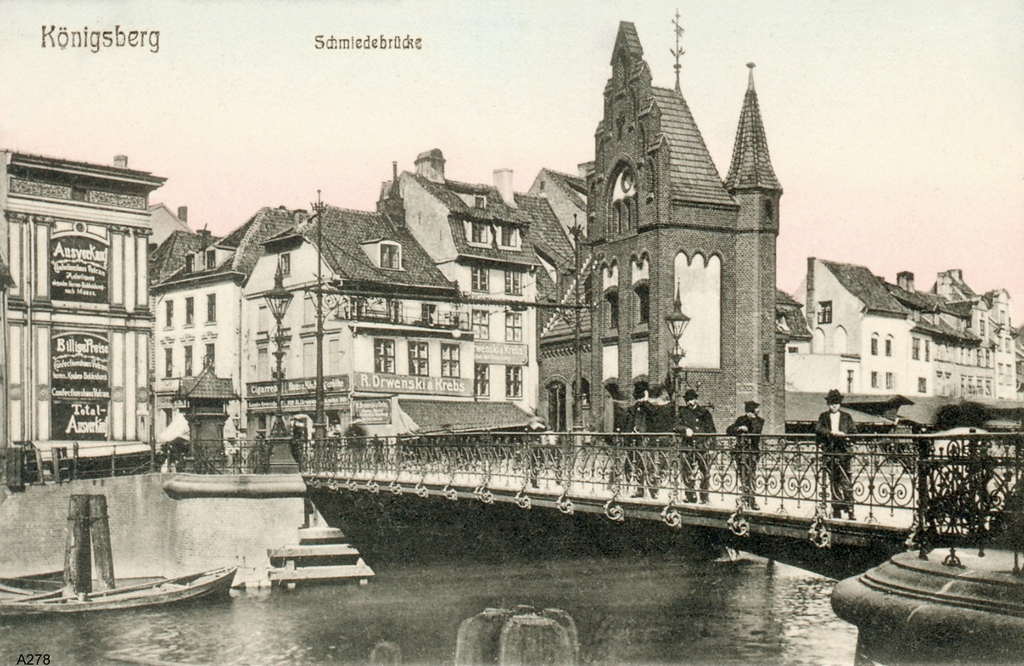
\includegraphics[width=0.6\paperwidth]{fig/konigsberg.jpg}
        \vspace{-0.25cm}
	    \caption{É possível fazer uma rota que atravesse todas as pontes sem repetir nenhuma?}
    \end{figure}
\end{frame}
%%% SLIDE %%%

%%% SLIDE %%%
\begin{frame}{Sete pontes de Königsberg}
    \only<1>{
        \begin{figure}
            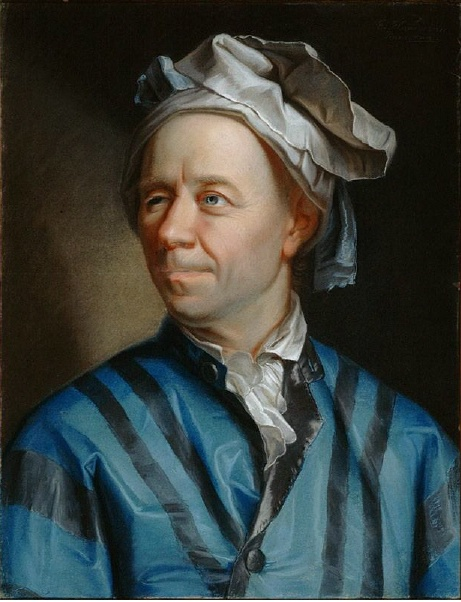
\includegraphics[width=0.3\paperwidth]{fig/euler.jpg}
            \vspace{-0.25cm}
	        \caption{Leonhard Euler (1707-1783)}
        \end{figure}
    }

    \only<2>{
        \begin{figure}
            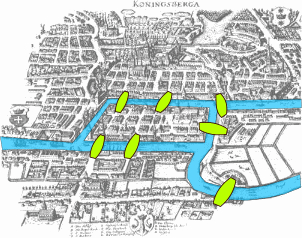
\includegraphics[width=0.5\paperwidth]{fig/bridges0.jpg}
        \end{figure}
    }

    \only<3>{
        \begin{figure}
            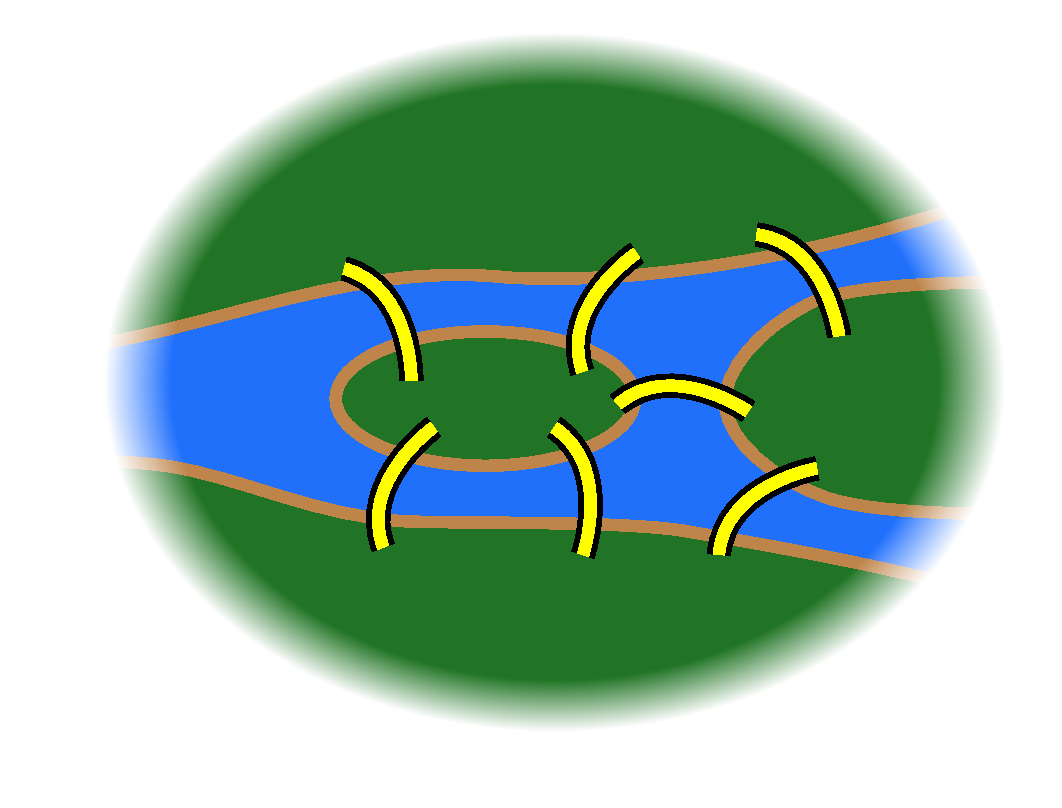
\includegraphics[width=0.5\paperwidth]{fig/bridges1.pdf}
        \end{figure}
    }
    
    \only<4>{
        \begin{figure}
            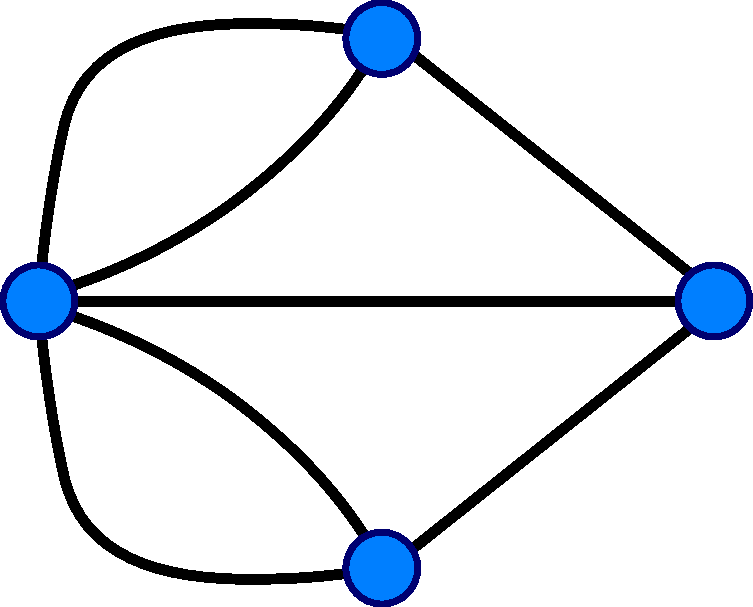
\includegraphics[width=0.5\paperwidth]{fig/bridges2.pdf}
        \end{figure}
    }
\end{frame}
%%% SLIDE %%%

%%% SLIDE %%%
\begin{frame}{Sete pontes de Königsberg}
    \begin{flushleft}
        Em 1736, Euler publicou um artigo com a solução do problema:
        
        \begin{itemize}
            \item Vínculos:
            \begin{itemize}
                \item Os pontos inicial e final da rota devem ter um número ímpar de pontes;
                \item Os pontos intermediários da rota devem possuir um número par de pontes.
            \end{itemize}
            
            \item Conclusões:
            \begin{itemize}
                \item Todos os pontos tem um número ímpar de pontes;
                \item Logo, a resposta do problema é {\bf NÃO}.
            \end{itemize}
        \end{itemize}
    \end{flushleft}
\end{frame}
%%% SLIDE %%%

%%% SLIDE %%%
\begin{frame}{O que são grafos?}
    \only<1>{
        \begin{center}
            \Large Grafos são entes matemáticos formados por dois conjuntos: Um
            de vértices e outro de arestas.
        \end{center}
    }
    
    \only<2>{
        Formalmente, podem ser representados como:
        \begin{equation}
            G(V,E)\nonumber
        \end{equation}
        
        onde,
        \begin{equation}
            V=\{v_1,v_2,\dots,v_n\}
            \quad\text{e}\quad
            E=\{e_1,e_2,\dots,e_m\}.
            \nonumber
        \end{equation}
    }
	
	\only<3>{
	    \begin{minipage}{0.45\textwidth}
		    \begin{figure}
			    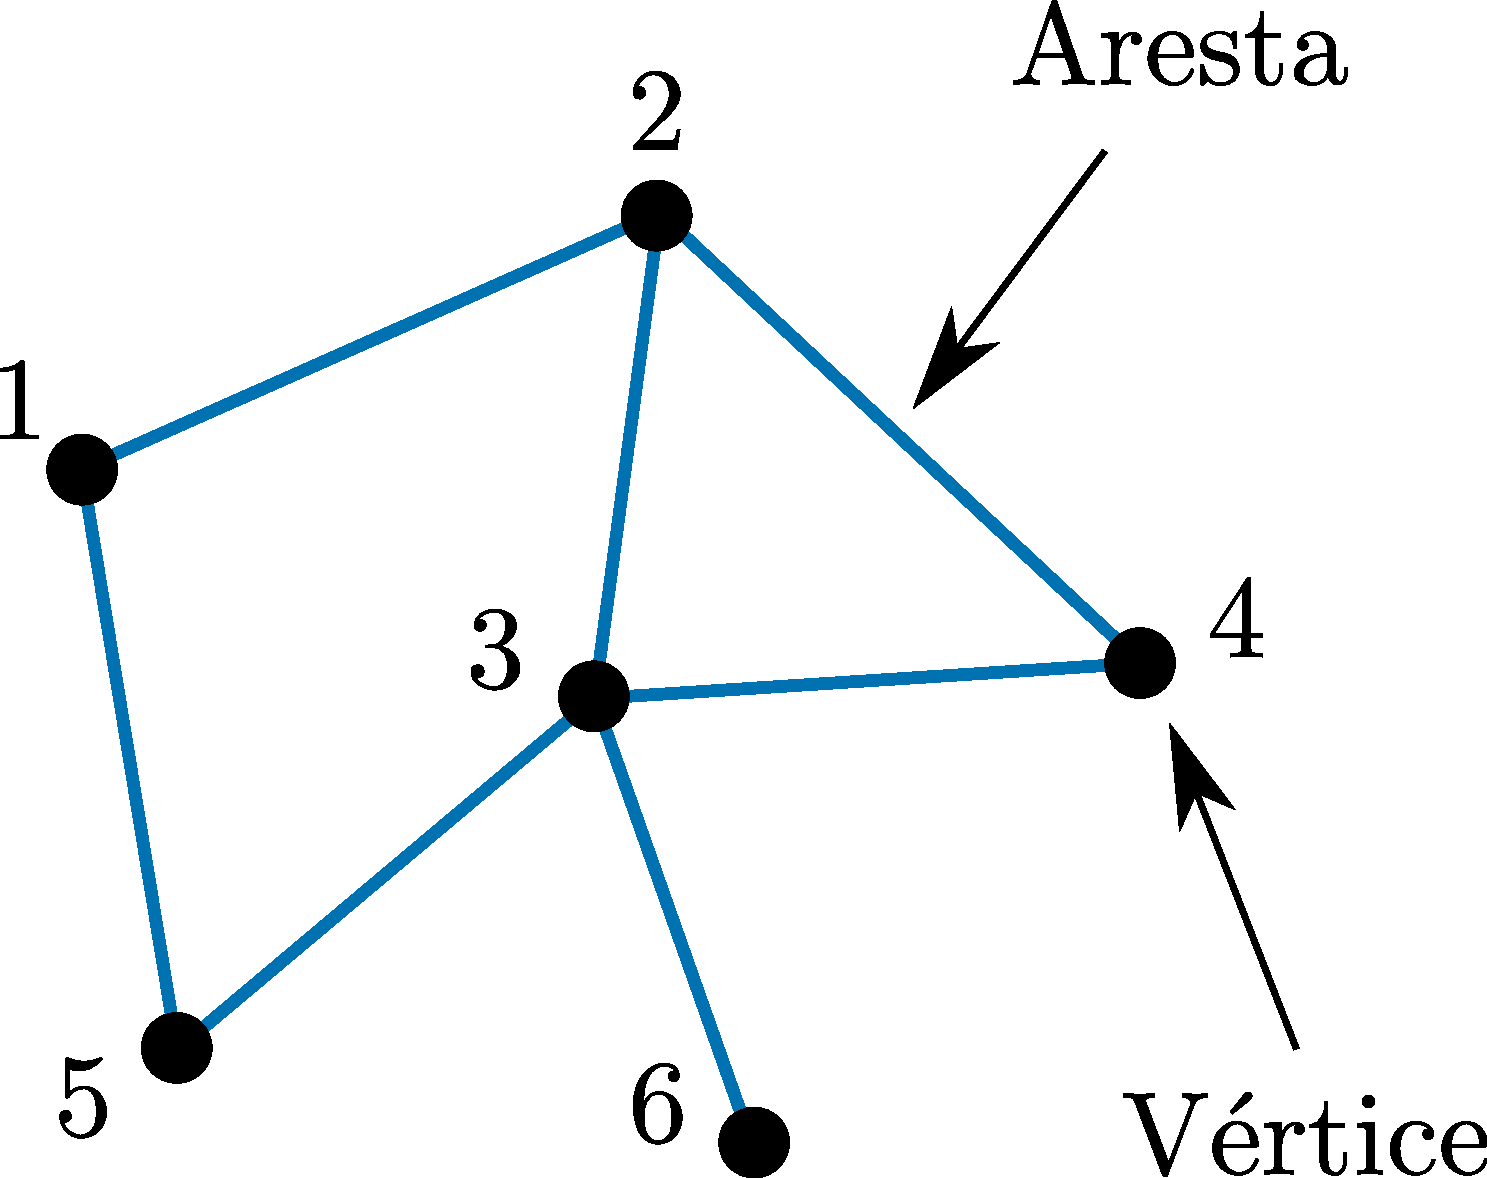
\includegraphics[width=0.4\paperwidth]{fig/graph.pdf}
			    \caption{Grafo Simples}
		    \end{figure}
	    \end{minipage}
	    \hspace{0.5cm}
	    \begin{minipage}{0.45\textwidth}
	        Matriz adjacência:
		    \begin{equation}
			    \mathbf{A} =
			    \begin{bmatrix}
				    0 & 1 & 0 & 0 & 1 & 0\\
				    1 & 0 & 1 & 1 & 0 & 0\\
				    0 & 1 & 0 & 1 & 1 & 1\\
				    0 & 1 & 1 & 0 & 0 & 0\\
				    1 & 0 & 1 & 0 & 0 & 0\\
				    0 & 0 & 1 & 0 & 0 & 0
			    \end{bmatrix}
			    .\nonumber
		    \end{equation}
	        Grau do vértice $i$:
	        \begin{equation}
	            k_i = \sum_{j=1}^{n} A_{ij} = \sum_{i=1}^{n} A_{ij}.
	            \nonumber
	        \end{equation}
	    \end{minipage}
	}
	
	\only<4>{
	    \begin{minipage}{0.45\textwidth}
		    \begin{figure}
			    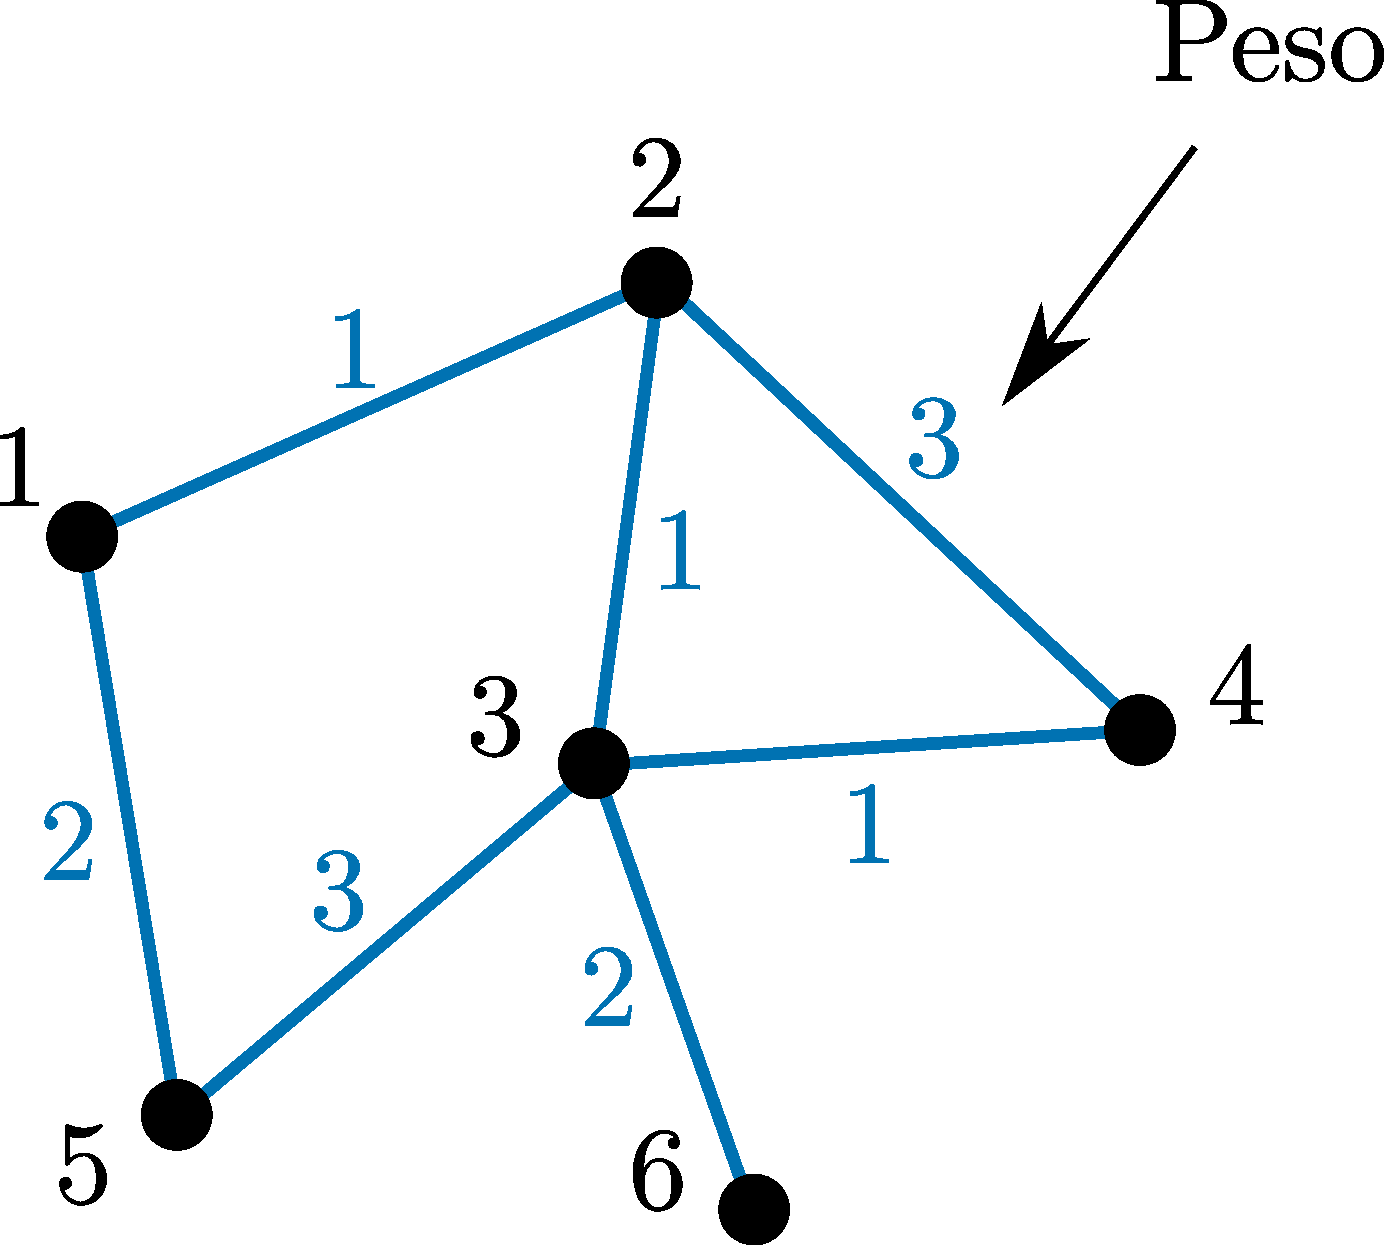
\includegraphics[width=0.4\paperwidth]{fig/weighted_graph.pdf}
			    \caption{Grafo Simples Ponderado}
		    \end{figure}
	    \end{minipage}
	    \hspace{0.5cm}
	    \begin{minipage}{0.45\textwidth}
	        Matriz adjacência:
		    \begin{equation}
			    \mathbf{A} =
			    \begin{bmatrix}
				    0 & 1 & 0 & 0 & 2 & 0\\
				    1 & 0 & 1 & 3 & 0 & 0\\
				    0 & 1 & 0 & 1 & 3 & 2\\
				    0 & 3 & 1 & 0 & 0 & 0\\
				    2 & 0 & 3 & 0 & 0 & 0\\
				    0 & 0 & 2 & 0 & 0 & 0
			    \end{bmatrix}
			    .\nonumber
		    \end{equation}
		    Grau ponderado do vértice $i$:
	        \begin{equation}
	            k_i = \sum_{j=1}^{n} A_{ij} = \sum_{i=1}^{n} A_{ij}.
	            \nonumber
	        \end{equation}
	    \end{minipage}
	}
	
	\only<5>{
		\begin{minipage}{0.45\textwidth}
			\begin{figure}
				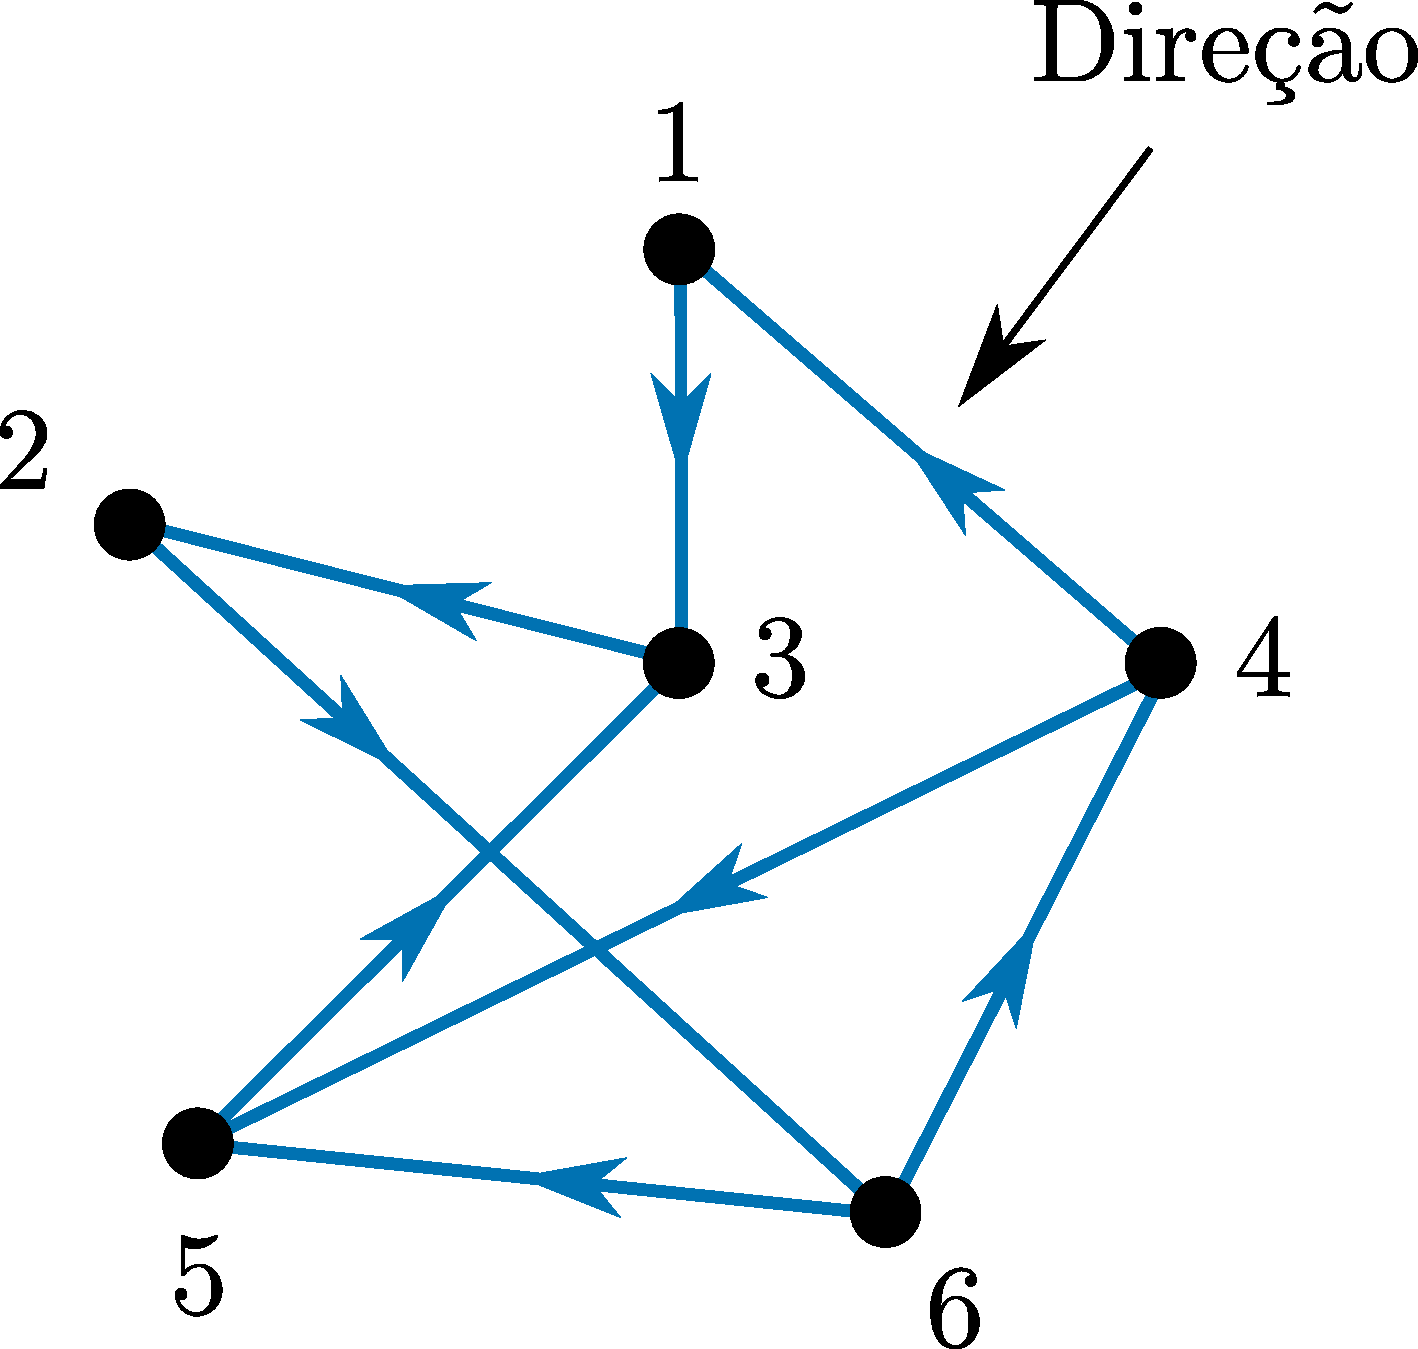
\includegraphics[width=0.4\paperwidth]{fig/digraph.pdf}
				\caption{Dígrafo Simples}
			\end{figure}
		\end{minipage}
		\hspace{0.5cm}
		\begin{minipage}{0.45\textwidth}
			Matriz adjacência:
			\begin{equation}
			    \mathbf{A} =
			    \begin{bmatrix}
				    0 & 0 & 0 & 1 & 0 & 0\\
				    0 & 0 & 1 & 0 & 0 & 0\\
				    1 & 0 & 0 & 0 & 1 & 0\\
				    0 & 0 & 0 & 0 & 0 & 1\\
				    0 & 0 & 0 & 1 & 0 & 1\\
				    0 & 1 & 0 & 0 & 0 & 0
			    \end{bmatrix}
			    .\nonumber
		    \end{equation}
		
		    Graus de entrada e de saída do vértice $i$:
	        \begin{equation}
	            k_i^{in} = \sum_{j=1}^{n} A_{ij}
	            \quad \text{e} \quad
	            k_i^{out} = \sum_{i=1}^{n} A_{ij}.
	            \nonumber
	        \end{equation}		
		\end{minipage}
	}
	
	\only<6>{
		\begin{minipage}{0.45\textwidth}
			\begin{figure}
				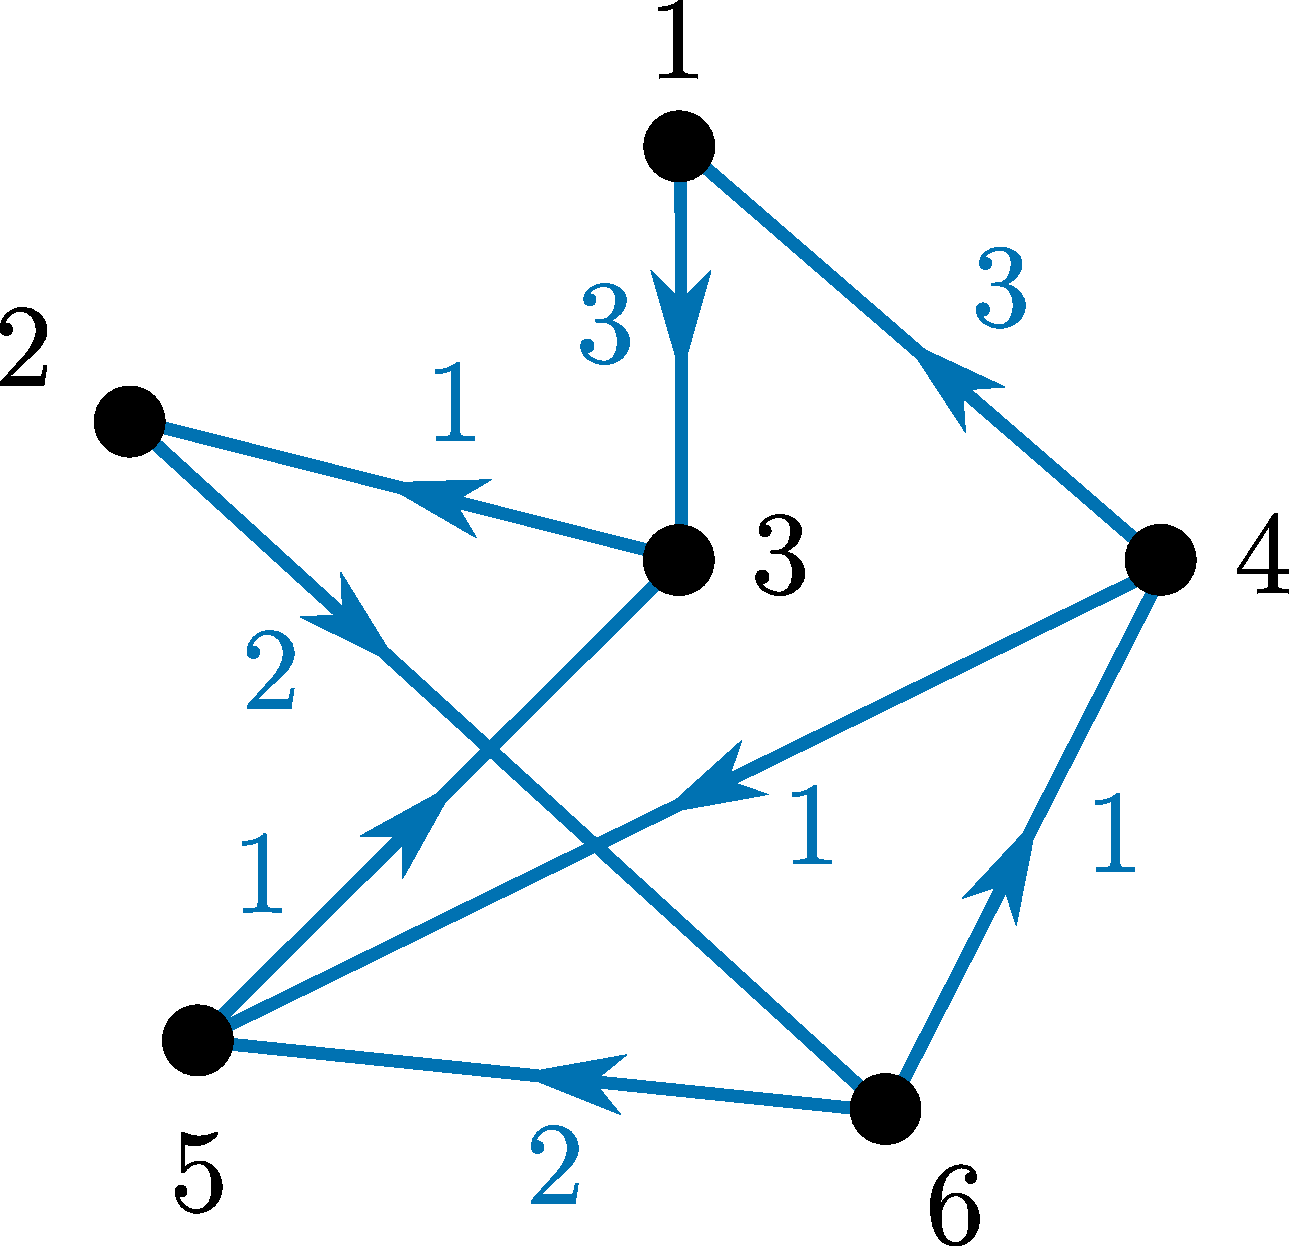
\includegraphics[width=0.4\paperwidth]{fig/weighted_digraph.pdf}
				\caption{Dígrafo Simples Ponderado}
			\end{figure}
		\end{minipage}
		\hspace{0.5cm}
		\begin{minipage}{0.45\textwidth}
			Matriz adjacência:
			\begin{equation}
			    \mathbf{A} =
			    \begin{bmatrix}
				    0 & 0 & 0 & 3 & 0 & 0\\
				    0 & 0 & 1 & 0 & 0 & 0\\
				    3 & 0 & 0 & 0 & 1 & 0\\
				    0 & 0 & 0 & 0 & 0 & 1\\
				    0 & 0 & 0 & 1 & 0 & 2\\
				    0 & 2 & 0 & 0 & 0 & 0
			    \end{bmatrix}
			    .\nonumber
		    \end{equation}
		    
		    Graus ponderados de entrada e saída do vértice $i$:
	        \begin{equation}
	            k_i^{in} = \sum_{j=1}^{n} A_{ij}
	            \quad \text{e} \quad
	            k_i^{out} = \sum_{i=1}^{n} A_{ij}.
	            \nonumber
	        \end{equation}	
		\end{minipage}
	}
\end{frame}
%%% SLIDE %%%

%%% SLIDE %%%
\begin{frame}{Outros tipos de grafos}
    \only<1>{
        \begin{minipage}{0.45\textwidth}
            \begin{figure}
                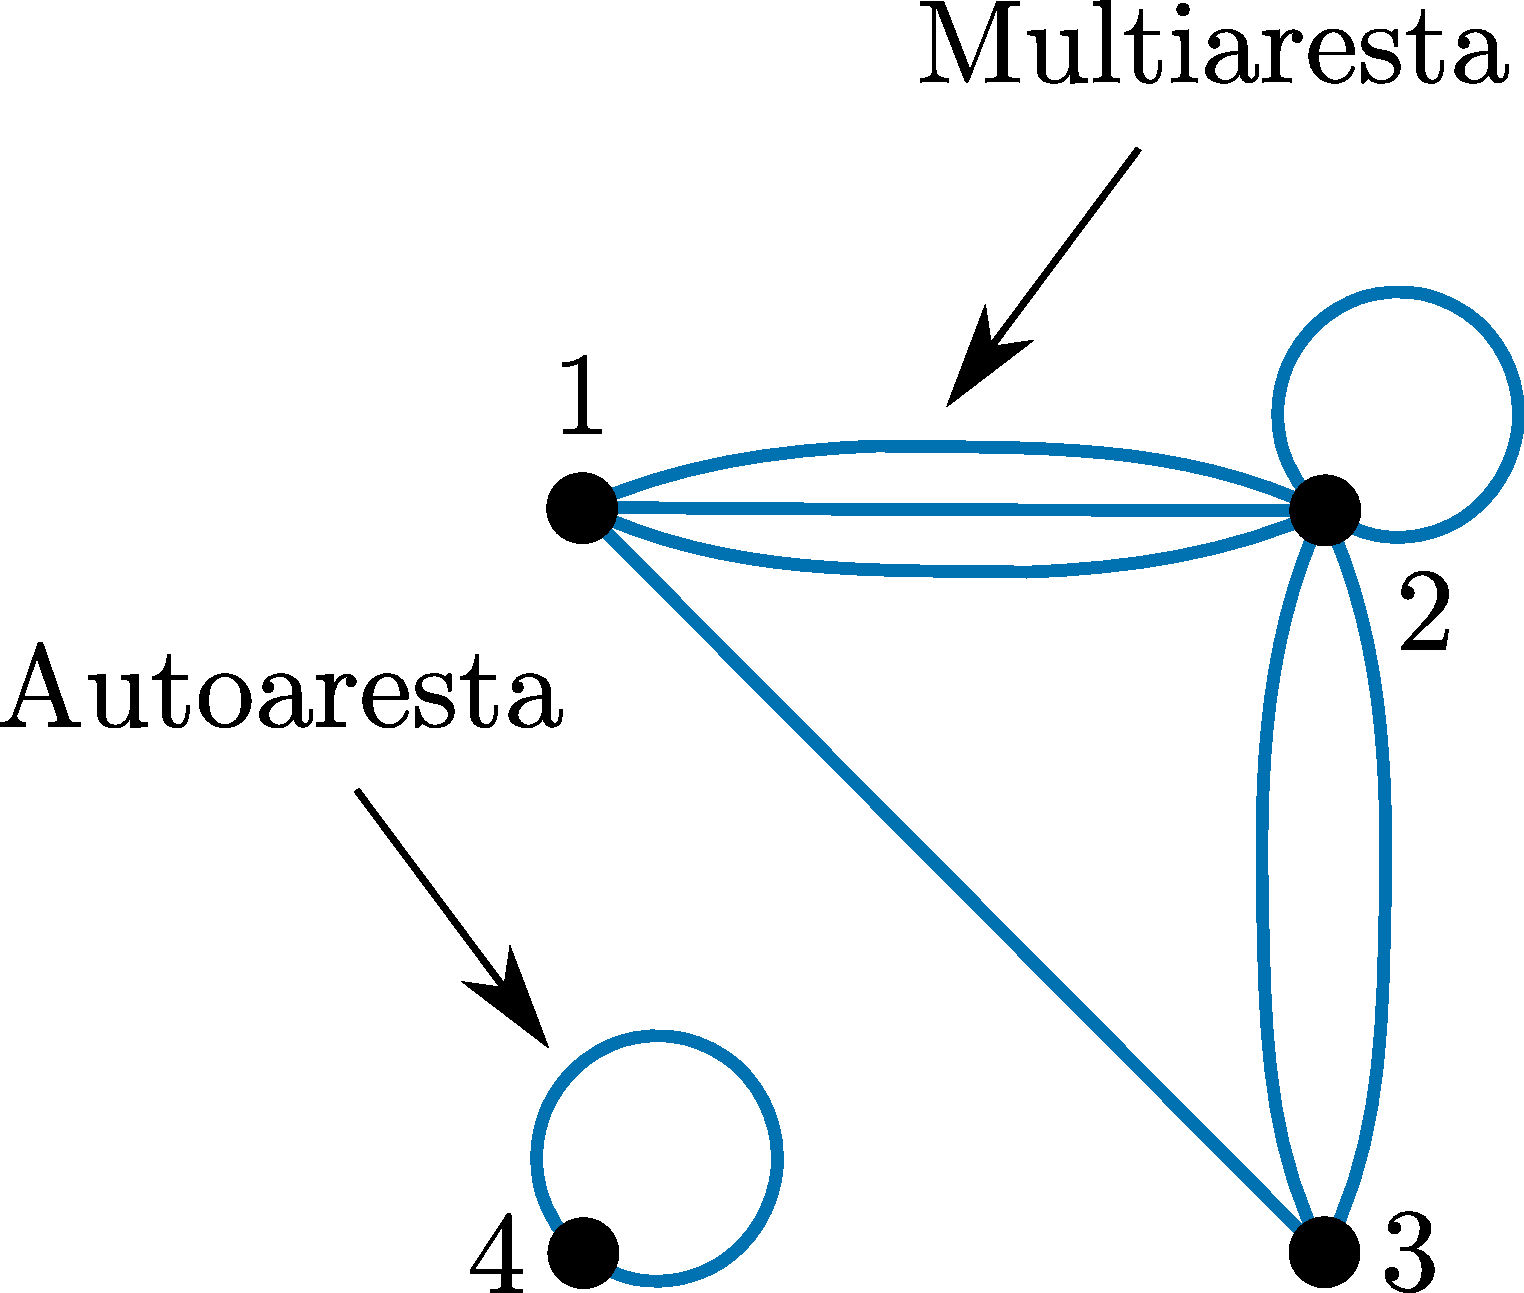
\includegraphics[width=0.4\paperwidth]{fig/multigraph.pdf}
                \caption{Multigrafo}
            \end{figure}
        \end{minipage}
        \hspace{0.5cm}
        \begin{minipage}{0.45\textwidth}
            \begin{figure}
                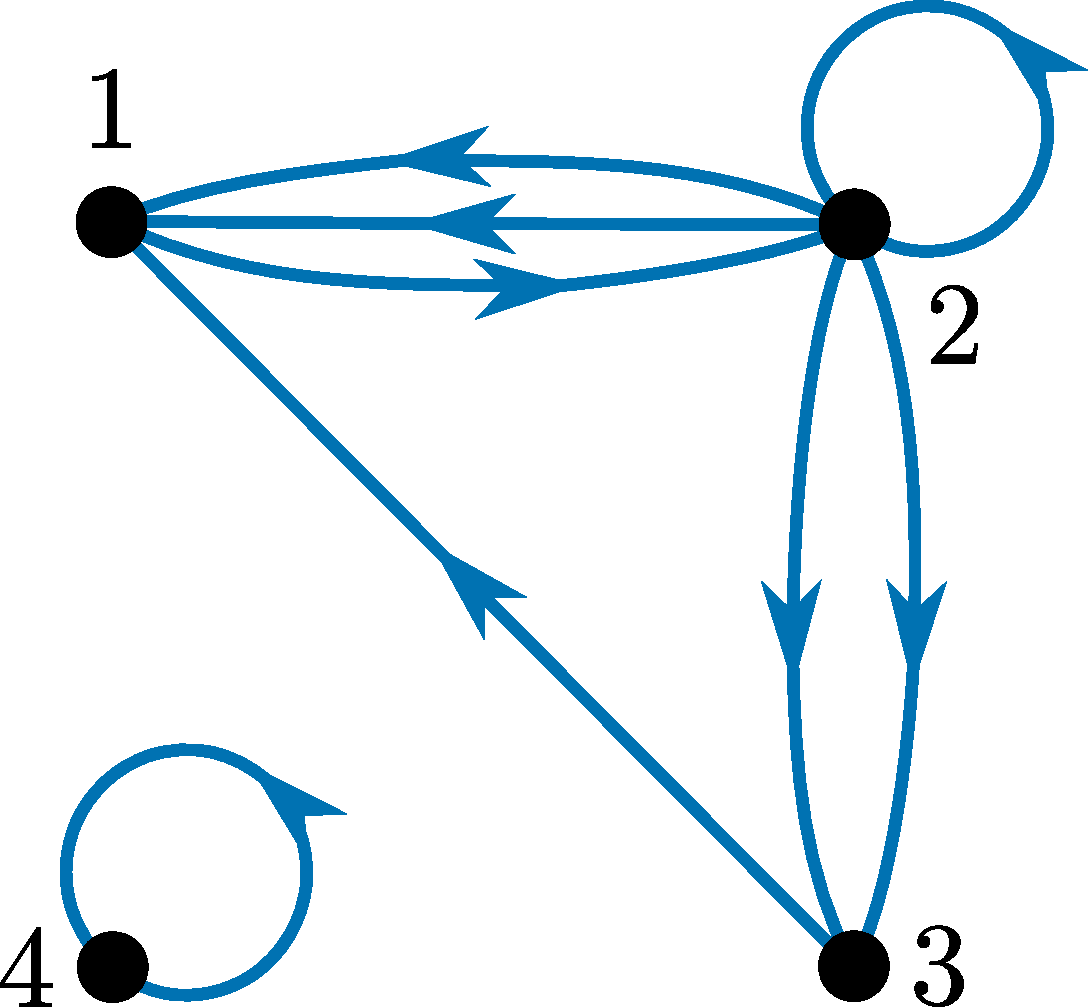
\includegraphics[width=0.4\paperwidth]{fig/multidigraph.pdf}
                \caption{Multidígrafo}
            \end{figure}
        \end{minipage}
    }
    
    \only<2>{
        \begin{minipage}{0.45\textwidth}
            \begin{figure}
                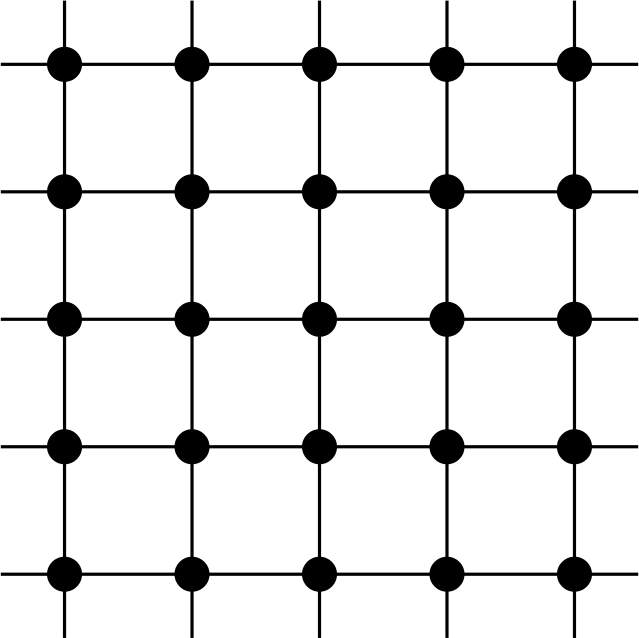
\includegraphics[width=0.3\paperwidth]{fig/regular_graph.jpg}
                \caption{Grafo Regular}
            \end{figure}
        \end{minipage}
        \hspace{0.5cm}
        \begin{minipage}{0.45\textwidth}
            \begin{figure}
                \includegraphics[width=0.3\paperwidth]{fig/complete_graph.pdf}
                \caption{Grafo Completo}
            \end{figure}
        \end{minipage}
    }
    
    \only<3>{
        \begin{minipage}{0.45\textwidth}
            \begin{figure}
                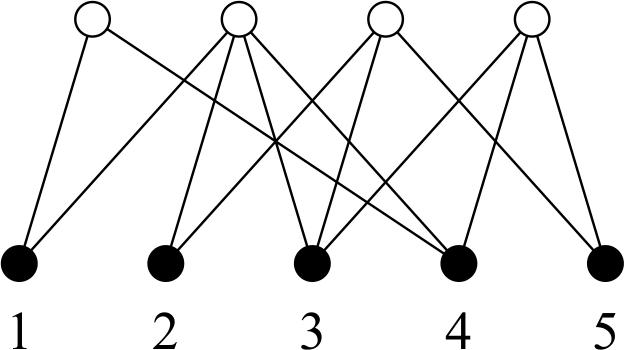
\includegraphics[width=0.4\paperwidth]{fig/bipartite_graph.jpg}
                \caption{Grafo Bipartido}
            \end{figure}
        \end{minipage}
        \hspace{0.5cm}
        \begin{minipage}{0.45\textwidth}
            \begin{figure}
                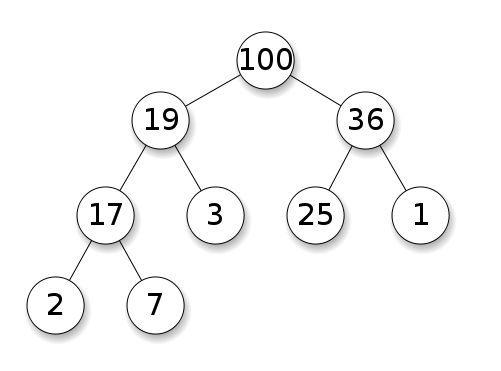
\includegraphics[width=0.4\paperwidth]{fig/tree_graph.jpg}
                \caption{Grafo Árvore}
            \end{figure}
        \end{minipage}
    }
    
    \only<4>{
        \begin{figure}
            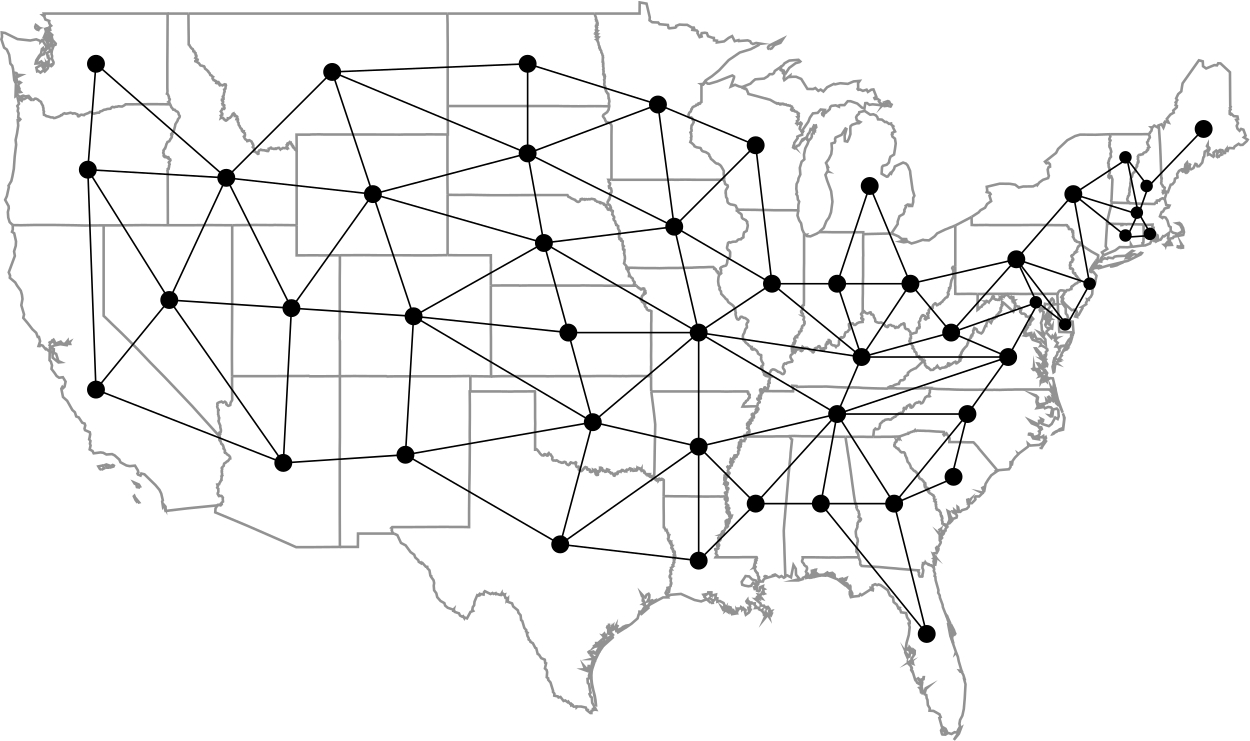
\includegraphics[width=0.6\paperwidth]{fig/planar_graph.jpg}
            \caption{Grafo Planar}
        \end{figure}
    }
\end{frame}
%%% SLIDE %%%

%%% SLIDE %%%
\begin{frame}{O que são redes complexas?}
	\only<1>{
		\begin{center}
			\Large Redes Complexas são abstrações que buscam quantificar as
			interações entre os elementos de um conjunto.
		\end{center}
	}
	
	\only<2>{
		\begin{figure}
			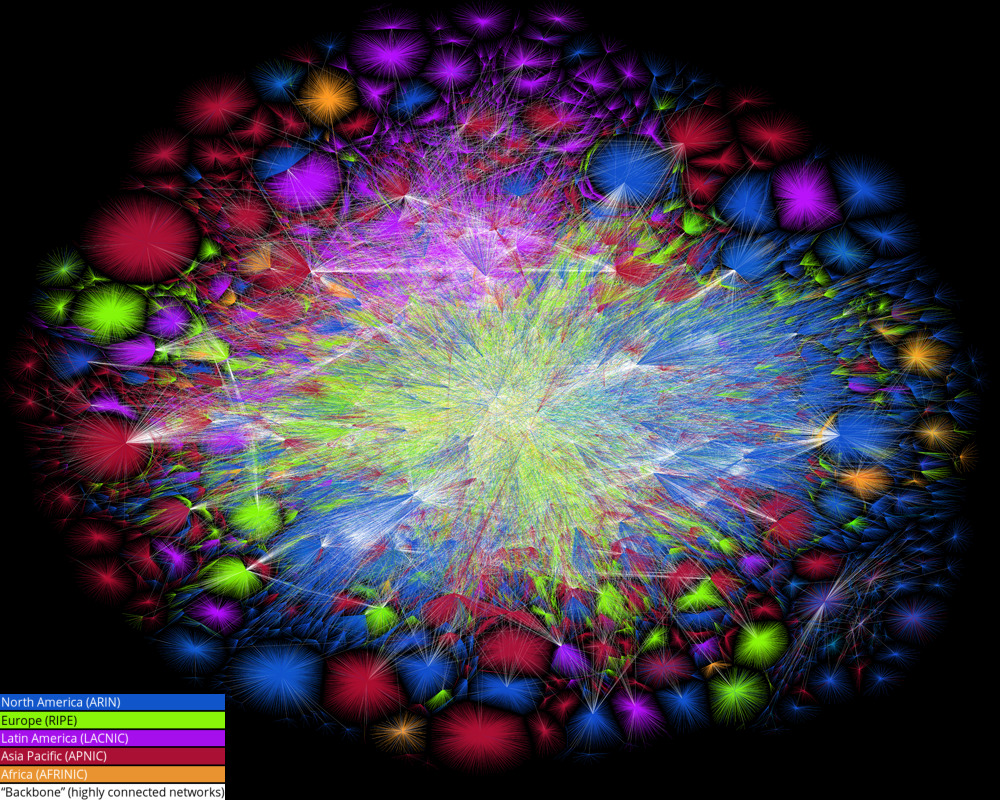
\includegraphics[width=0.55\paperwidth]{fig/internet.jpg}
		\end{figure}
	}
\end{frame}
%%% SLIDE %%%

%%% SLIDE %%%
\begin{frame}{E qual é a diferença?}
	\begin{center}
		\Large Nenhuma! Redes Complexas são grafos com um grande número de
		elementos e propriedades topológicas não-triviais.
	\end{center}
\end{frame}
%%% SLIDE %%%

%%% SLIDE %%%
\begin{frame}{Exemplos: Redes Tecnológicas}	
	\only<1>{
		\begin{figure}
			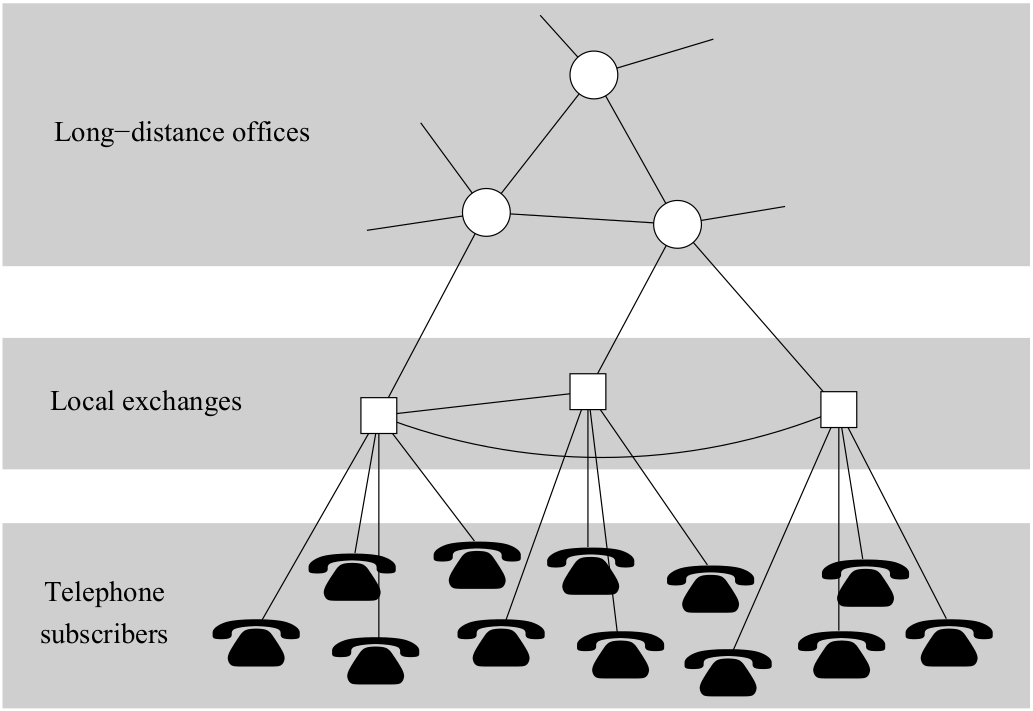
\includegraphics[width=0.6\paperwidth]{fig/telephone.jpg}
		\end{figure}
	}
	
	\only<2>{
		\begin{figure}
			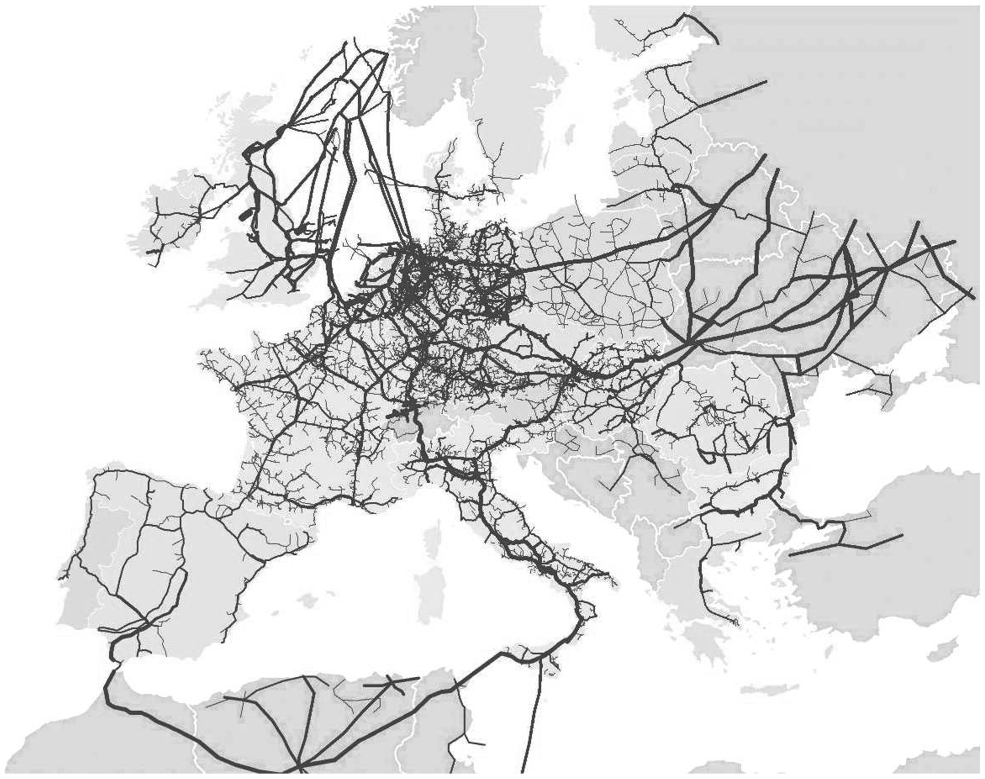
\includegraphics[width=0.55\paperwidth]{fig/pipelines.jpg}
		\end{figure}
	}
	
	\only<3>{
		\begin{center}
			\href{run:vid/volcano.mp4}{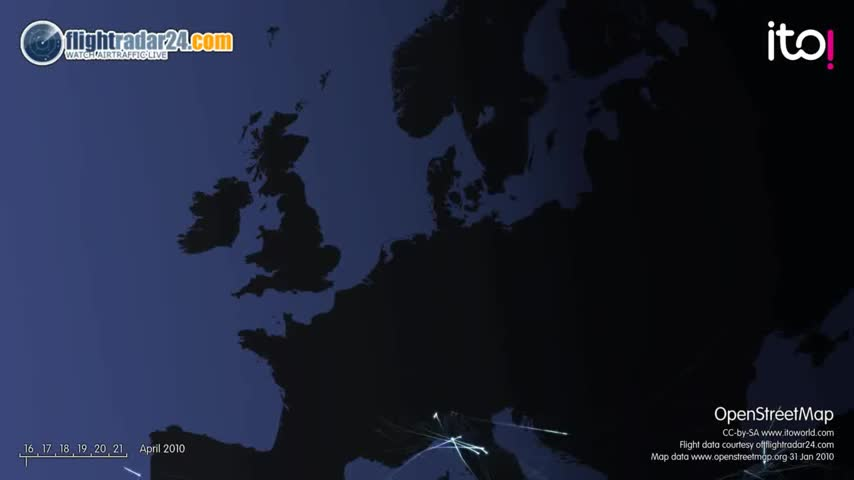
\includegraphics[width=0.8\textwidth]{vid/volcano.jpg}}
		\end{center}
	}
	
	\only<4>{
		\begin{figure}
			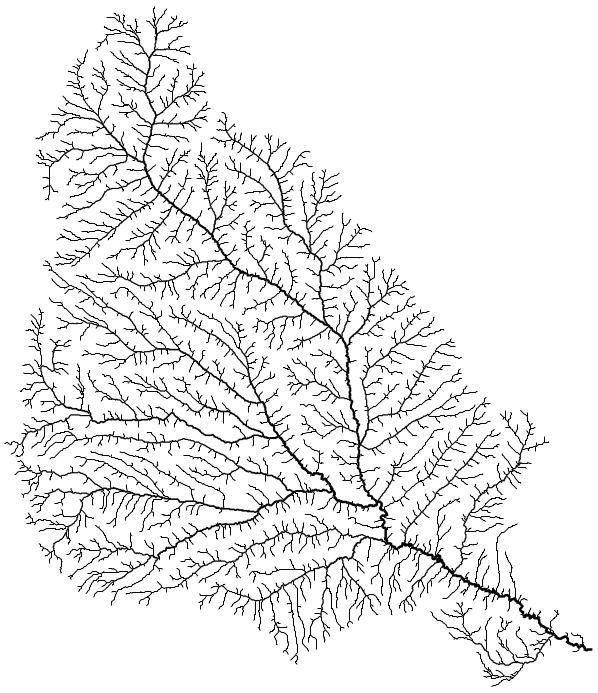
\includegraphics[width=0.35\paperwidth]{fig/river.jpg}
		\end{figure}
	}
\end{frame}
%%% SLIDE %%%

%%% SLIDE %%%
\begin{frame}{Exemplos: Redes Sociais}	
	\only<1>{
		\begin{figure}
			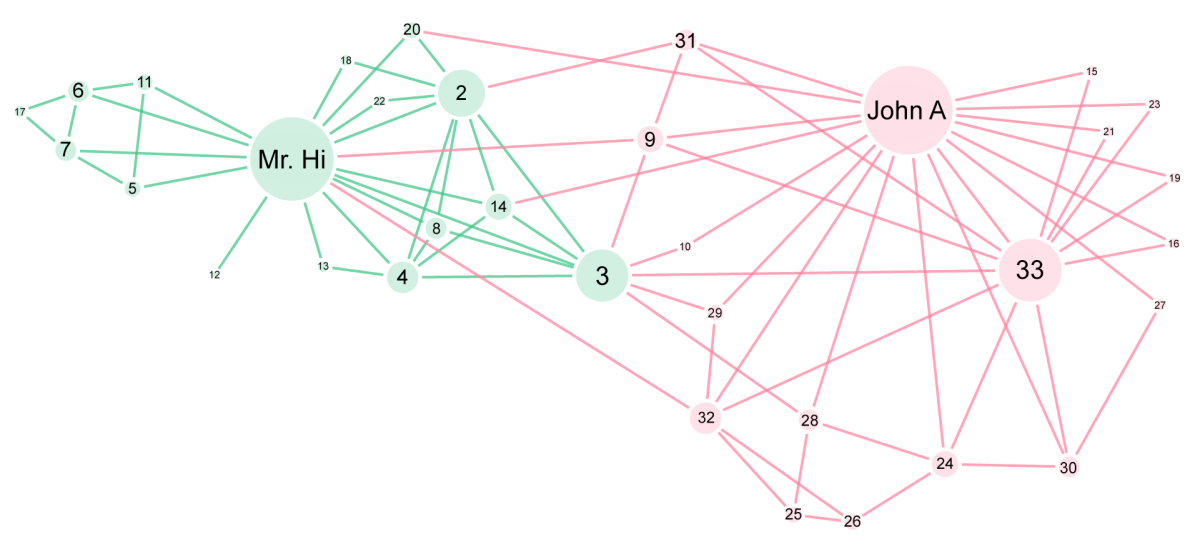
\includegraphics[width=0.8\paperwidth]{fig/karate_club.jpg}
		\end{figure}
	}
	
	\only<2>{
		\begin{figure}
			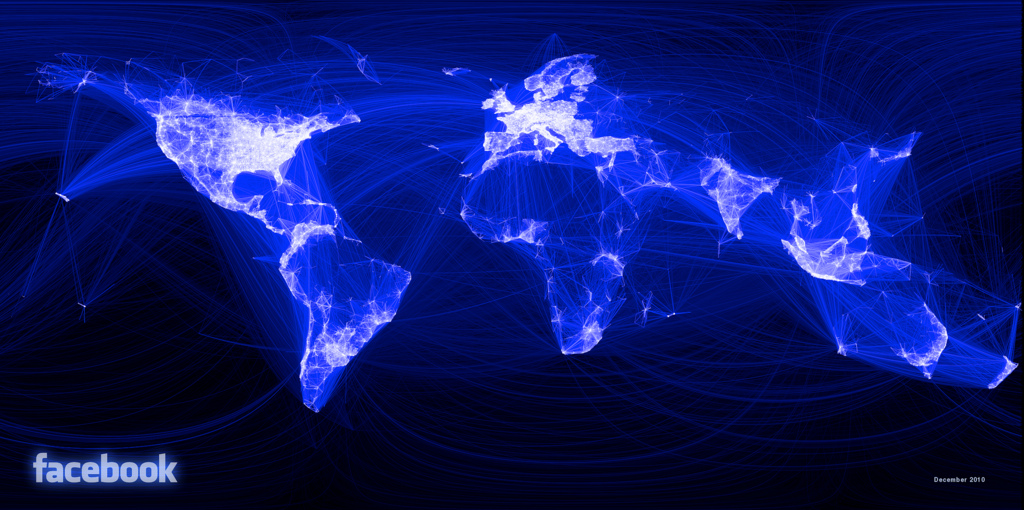
\includegraphics[width=0.9\paperwidth]{fig/facebook.jpg}
		\end{figure}
	}
\end{frame}
%%% SLIDE %%%

%%% SLIDE %%%
\begin{frame}{Exemplos: Redes de Informações}
	\only<1>{
		\begin{figure}
			
\includegraphics[width=0.65\paperwidth]{fig/fakenews.jpg}
		\end{figure}
	}
	
	\only<2>{
		\begin{figure}
			
\includegraphics[width=0.45\paperwidth]{fig/briga.jpg}
		\end{figure}
	}
\end{frame}
%%% SLIDE %%%

%%% SLIDE %%%
\begin{frame}{Exemplos: Redes Biológicas}
	\only<1>{
		\begin{figure}
			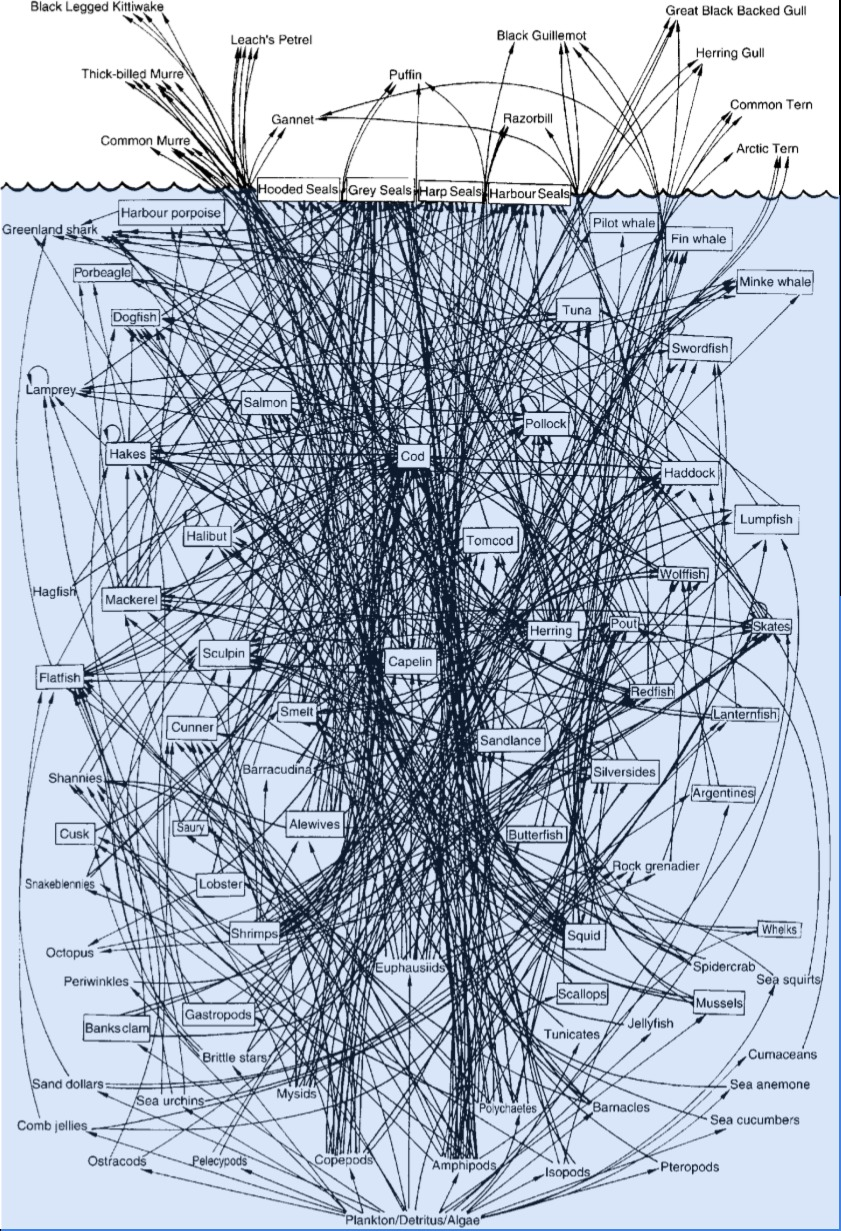
\includegraphics[width=0.3\paperwidth]{fig/foodweb.jpg}
		\end{figure}
	}
	
	\only<2>{
		\begin{figure}
			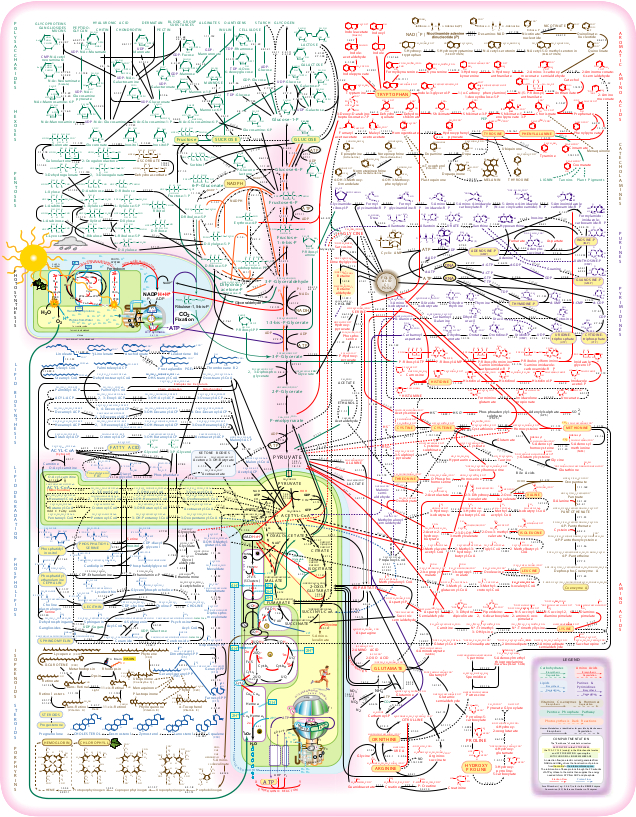
\includegraphics[width=0.3\paperwidth]{fig/metabolism.jpg}
		\end{figure}
	}
	
	\only<3>{
		\begin{center}
			\href{run:vid/fireflies.mp4}{
\includegraphics[width=0.55\textwidth]{vid/fireflies.jpg}}
		\end{center}
	}
	
	\only<4>{
		\begin{center}
			\href{run:vid/metronomes.mp4}{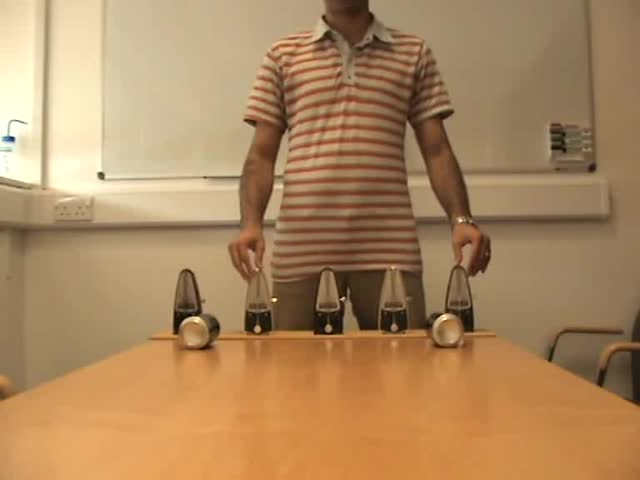
\includegraphics[width=0.6\textwidth]{vid/metronomes.jpg}}
		\end{center}
	}
\end{frame}
%%% SLIDE %%%

%%% SLIDE %%%
\begin{frame}{O que se usa para modelar redes complexas?}
    \begin{center}
        \begin{figure}
            
\includegraphics[width=0.5\paperwidth]{fig/networkx.pdf}
            \caption{\url{https://networkx.org/}}
        \end{figure}
        
        \begin{minipage}{0.40\textwidth}
            \begin{figure}
                
\includegraphics[width=0.4\paperwidth]{fig/graphtool.jpg}
                \caption{\url{https://graph-tool.skewed.de/}}
            \end{figure}
        \end{minipage}
        \hspace{0.5cm}
        \begin{minipage}{0.40\textwidth}
            \begin{figure}
                
\includegraphics[width=0.3\paperwidth]{fig/gephi.jpg}
                \caption{\url{https://gephi.org/}}
            \end{figure}
        \end{minipage}
    \end{center}
\end{frame}
%%% SLIDE %%%

%%% SLIDE %%%
\begin{frame}{Projeto de Redes Complexas}
    \only<1>{
	    \begin{figure}
		    
\includegraphics[width=0.7\paperwidth]{fig/got.jpg}
		    \caption{\href{https://genius.com/artists/Game-of-thrones}{https://genius.com/artists/Game-of-thrones}}
	    \end{figure}
	}
	
	\only<2>{
	    \begin{center}
	        \Huge Quem é o personagem principal da série?
	    \end{center}
	}
\end{frame}
%%% SLIDE %%%

%%% SLIDE %%%
\begin{frame}{Bibliografia}
    \begin{center}
        \begin{minipage}{0.25\textwidth}
            \begin{figure}
                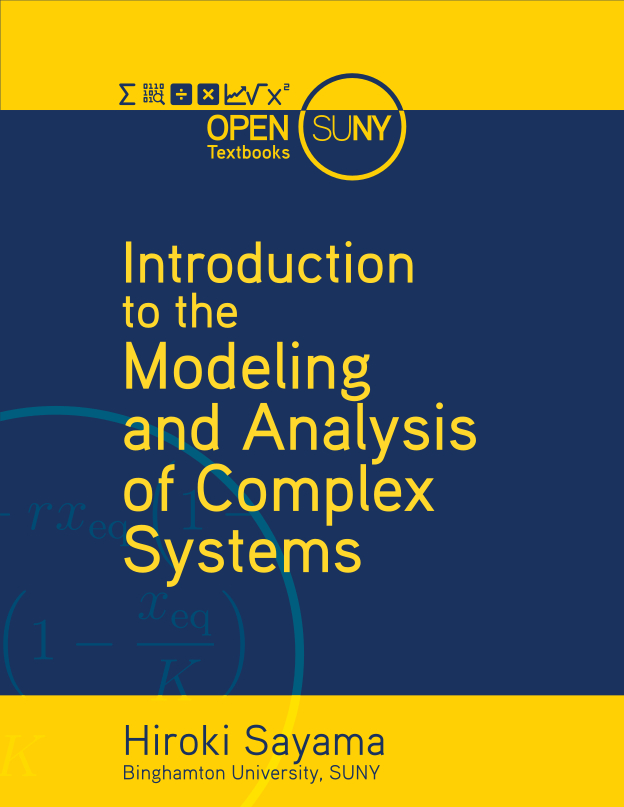
\includegraphics[width=0.25\paperwidth]{fig/textbook1.jpg}
            \end{figure}
        \end{minipage}
        \hspace{0.5cm}
        \begin{minipage}{0.25\textwidth}
            \begin{figure}
                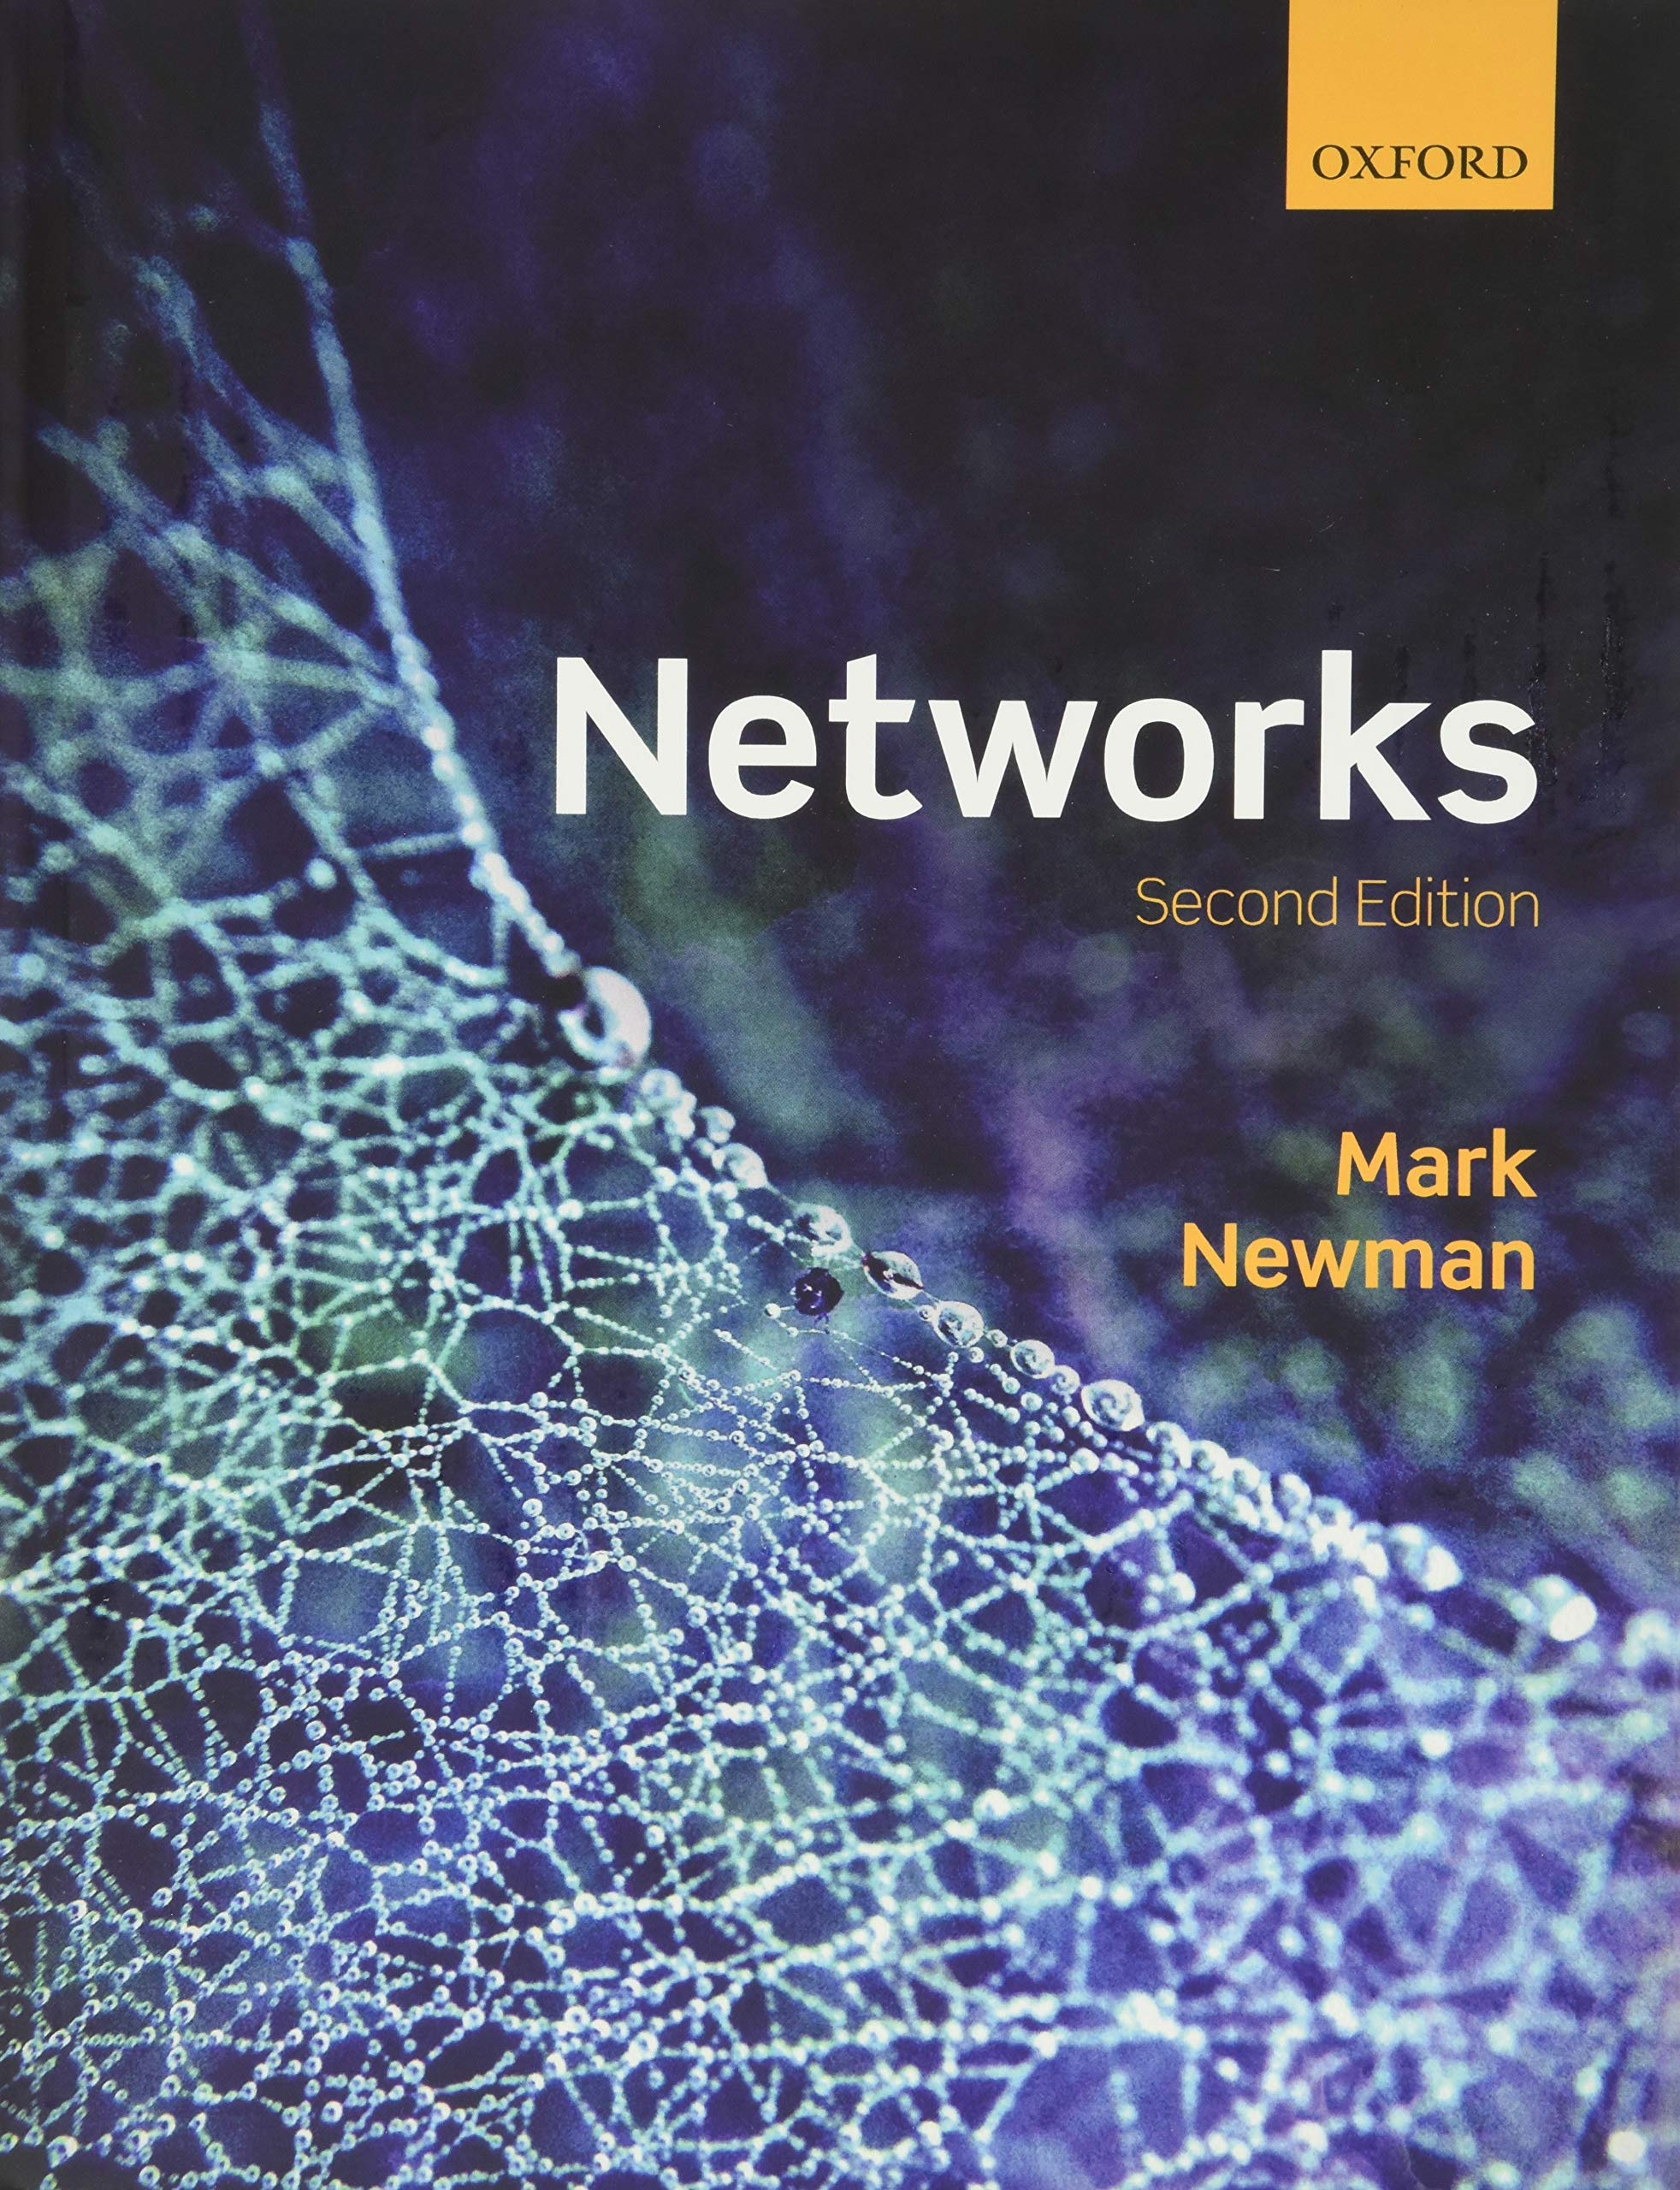
\includegraphics[width=0.25\paperwidth]{fig/textbook2.jpg}
            \end{figure}
        \end{minipage}
        \hspace{0.5cm}
        \begin{minipage}{0.25\textwidth}
            \begin{figure}
                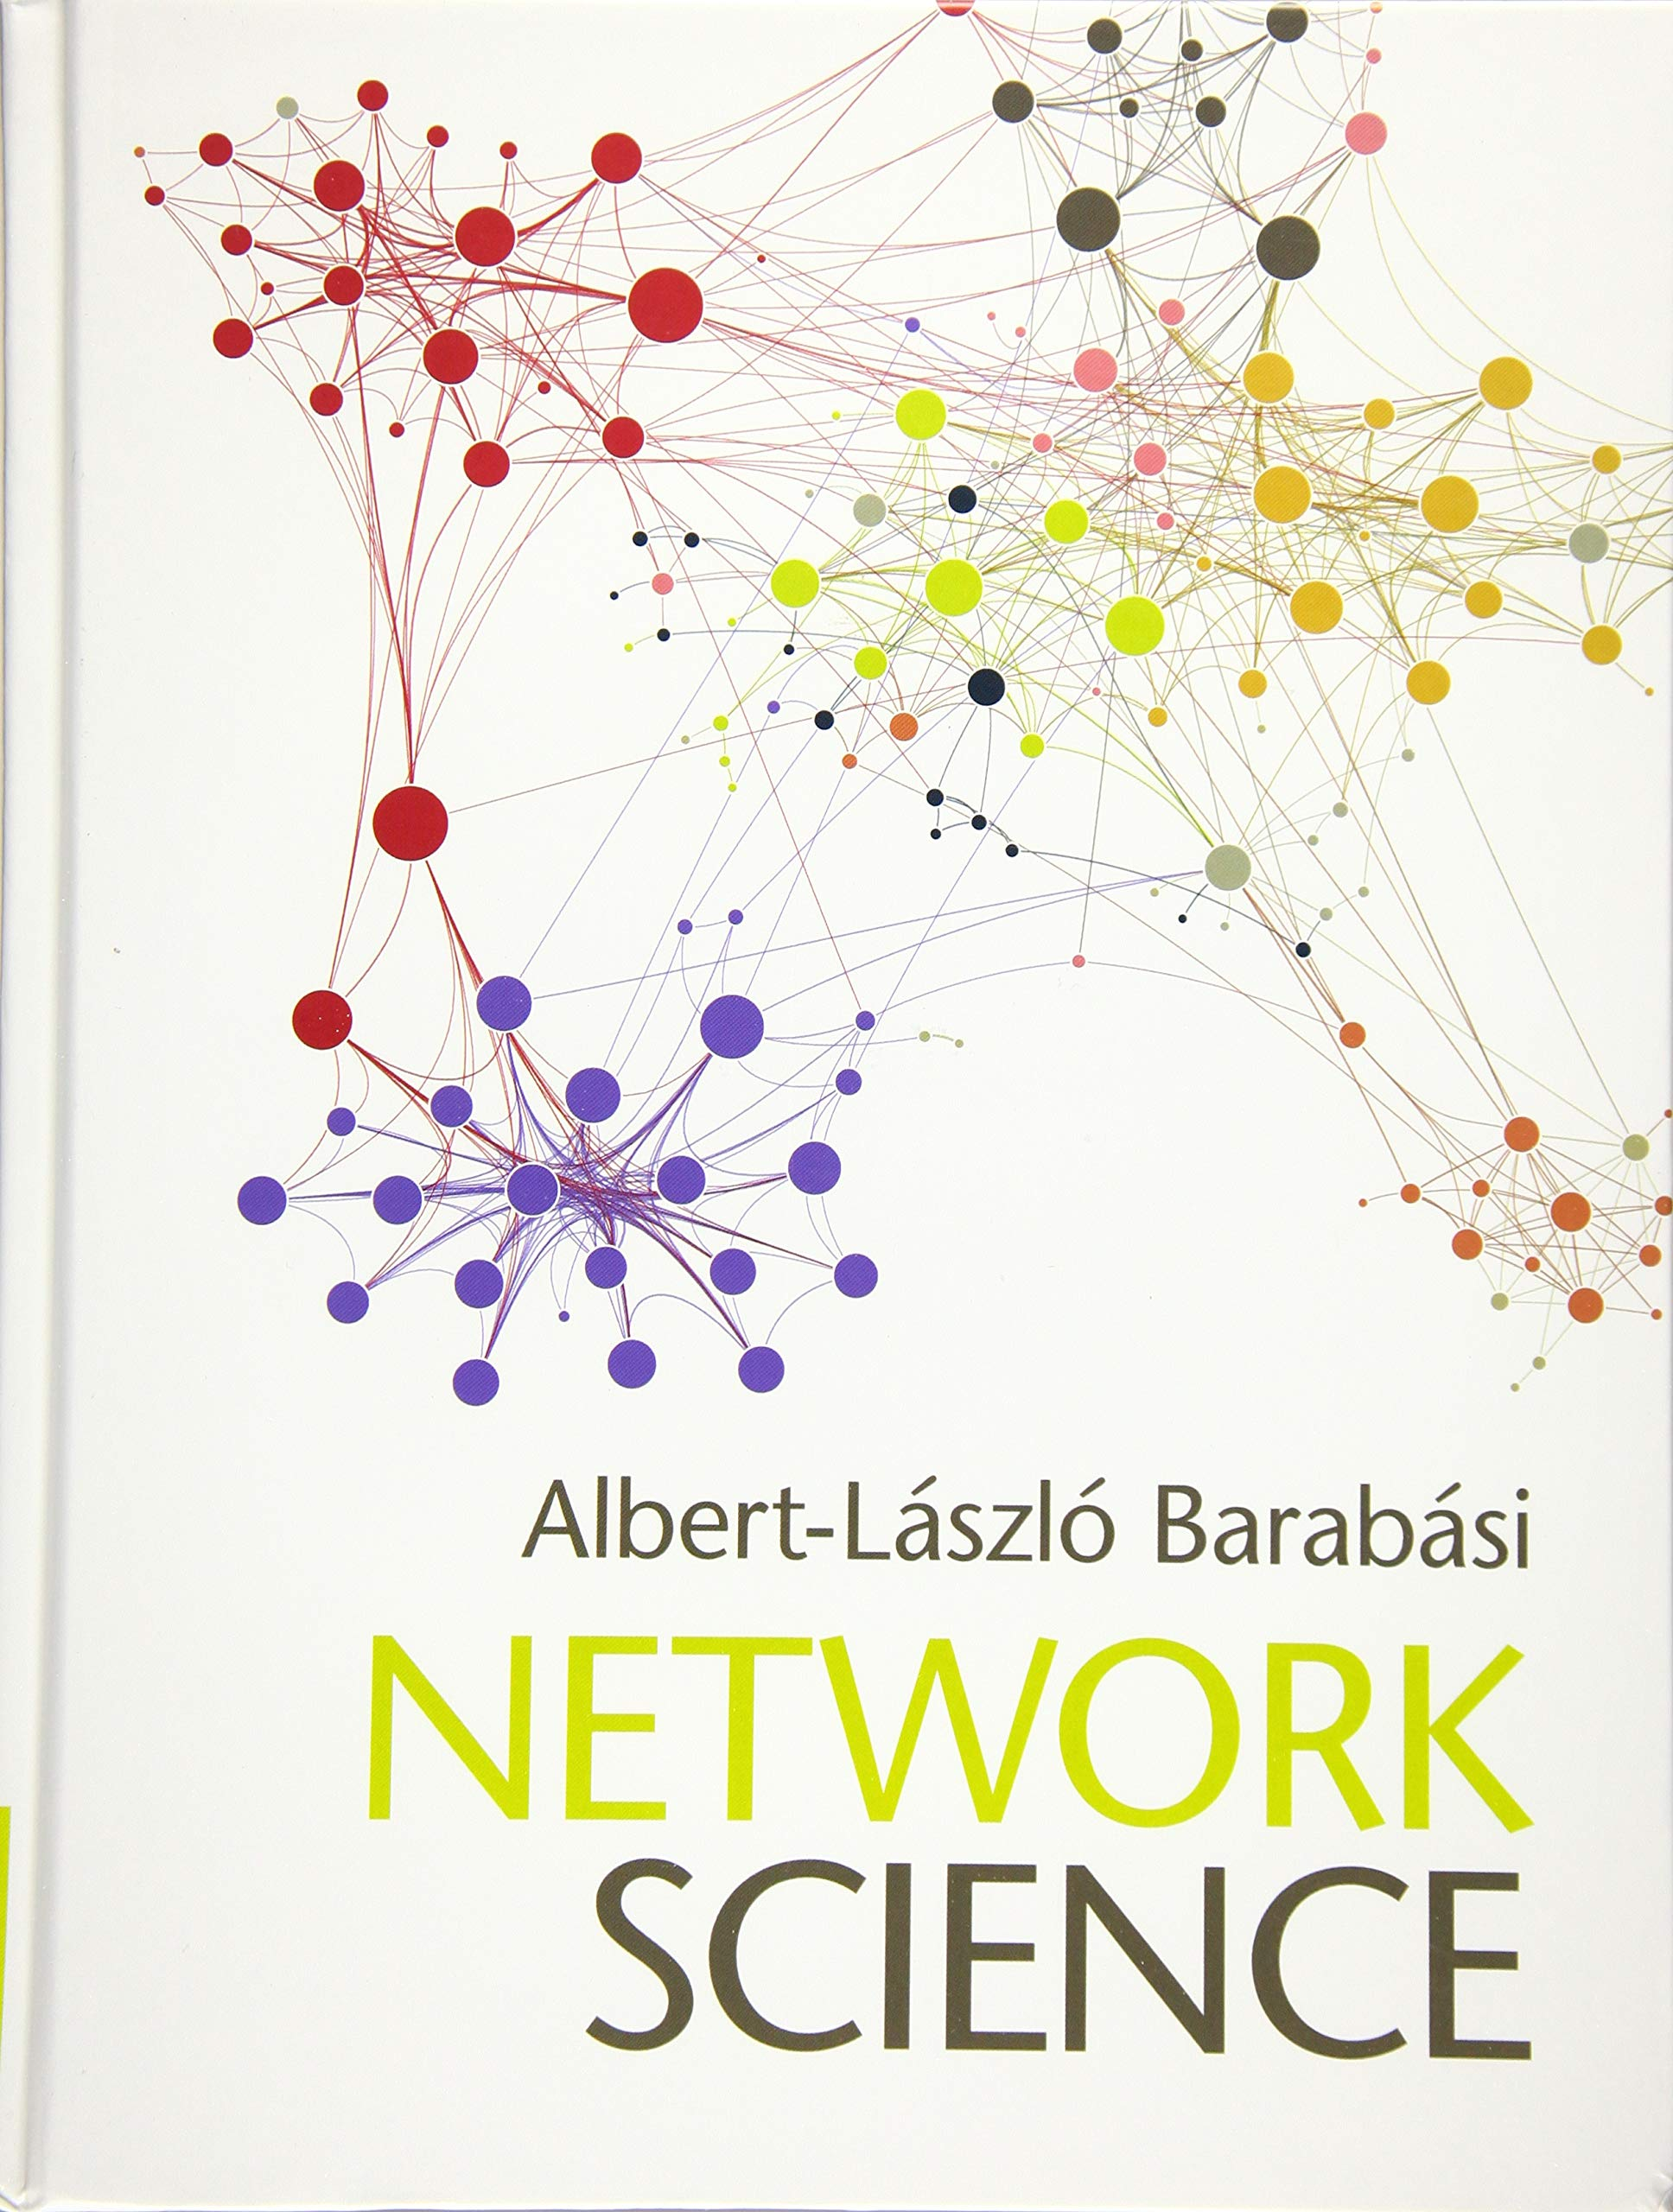
\includegraphics[width=0.25\paperwidth]{fig/textbook3.jpg}
            \end{figure}
        \end{minipage}
    \end{center}
\end{frame}
%%% SLIDE %%%

\end{document}
